%%%%%%%%%%%%%%%%%%%%%%%%%%%%%%%%%%%%%%%%%
% Template
% LaTeX Template
% Version 1.0 (December 8 2014)
%
% This template has been downloaded from:
% http://www.LaTeXTemplates.com
%
% Original author:
% Brandon Fryslie
% With extensive modifications by:
% Vel (vel@latextemplates.com)
%
% License:
% CC BY-NC-SA 3.0 (http://creativecommons.org/licenses/by-nc-sa/3.0/)
%
% Authors:
% Sabbir Ahmed, Jeffrey Osazuwa, Howard To, Brian Weber
% 
%%%%%%%%%%%%%%%%%%%%%%%%%%%%%%%%%%%%%%%%%

\documentclass[paper=usletter, fontsize=12pt]{article}
%%%%%%%%%%%%%%%%%%%%%%%%%%%%%%%%%%%%%%%%%
% Contract
% Structural Definitions File
% Version 1.0 (December 8 2014)
%
% Created by:
% Vel (vel@latextemplates.com)
% 
% This file has been downloaded from:
% http://www.LaTeXTemplates.com
%
% License:
% CC BY-NC-SA 3.0 (http://creativecommons.org/licenses/by-nc-sa/3.0/)
%
%%%%%%%%%%%%%%%%%%%%%%%%%%%%%%%%%%%%%%%%%

%----------------------------------------------------------------------------------------
%   PARAGRAPH SPACING SPECIFICATIONS
%----------------------------------------------------------------------------------------

\setlength{\parindent}{0mm} % Don't indent paragraphs

\setlength{\parskip}{2.5mm} % Whitespace between paragraphs

%----------------------------------------------------------------------------------------
%   PAGE LAYOUT SPECIFICATIONS
%----------------------------------------------------------------------------------------

\usepackage{geometry} % Required to modify the page layout
\usepackage{multicol}

\setlength{\textwidth}{16cm} % Width of the text on the page
\setlength{\textheight}{23cm} % Height of the text on the page

\setlength{\oddsidemargin}{0cm} % Width of the margin - negative to move text left, positive to move it right

% Uncomment for offset margins if the 'twoside' document class option is used
%\setlength{\evensidemargin}{-0.75cm} 
%\setlength{\oddsidemargin}{0.75cm}

\setlength{\topmargin}{-1.25cm} % Reduce the top margin

%-------------------------------------------

\usepackage[utf8]{inputenc} % Required for including letters with accents
\usepackage[T1]{fontenc} % Use 8-bit encoding that has 256 glyphs

\usepackage{avant} % Use the Avantgarde font for headings
\usepackage{mathptmx} % Use the Adobe Times Roman as the default text font together with math symbols from the Sym­bol, Chancery and Com­puter Modern fonts

%----------------------------------------------------------------------------------------
%   SECTION TITLE SPECIFICATIONS
%----------------------------------------------------------------------------------------

\usepackage{titlesec} % Required for modifying section titles

\titleformat{\section} % Customize the \section{} section title
{\sffamily\large\bfseries} % Title font customizations
{\thesection} % Section number
{16pt} % Whitespace between the number and title
{\large} % Title font size
\titlespacing*{\section}{0mm}{7mm}{0mm} % Left, top and bottom spacing around the title

\titleformat{\subsection} % Customize the \subsection{} section title
{\sffamily\normalsize\bfseries} % Title font customizations
{\thesubsection} % Subsection number
{16pt} % Whitespace between the number and title
{\normalsize} % Title font size
\titlespacing*{\subsection}{0mm}{5mm}{0mm} % Left, top and bottom spacing around the title
\renewcommand\familydefault{\sfdefault} % specifies the document layout and style

%----------------------------------------------------------------------------------------

% names
\newcommand{\team}{Galois Field Arithmetic Unit}
\newcommand{\Sabbir}{Sabbir Ahmed}
\newcommand{\Jeffrey}{Jeffrey Osazuwa}
\newcommand{\Howard}{Howard To}
\newcommand{\Brian}{Brian Weber}

% document info command
\newcommand{\documentinfo}[5]{
    \begin{centering}
        \parbox{2in}{
        \begin{spacing}{1}
            \begin{flushleft}
                \begin{tabular}{l l}
                    #1 \\
                    #2 \\
                    #3 \\
                    #4 \\
                    #5 \\
                \end{tabular}\\
                \rule{\textwidth}{1pt}
            \end{flushleft}
        \end{spacing}
        }
    \end{centering}
}

\begin{document}


    \documentinfo{\textbf{MEMO NUMBER:} 03}{\textbf{DATE:} \today}{\textbf{TO: } EFC LaBerge}{\textbf{FROM: }\Sabbir, \Jeffrey, \Howard, \Brian}{\textbf{SUBJECT: } System Requirement Specifications Draft}
    \vspace{-0.1in}

    \section{Introduction}
    A Galois field is a field with a finite number of elements. The nomenclature $GF(q)$ is used to indicate a Galois field with q elements. For $GF(q)$ in general, $q$ must be a power of a prime. For each prime power, there exists exactly one finite field. The best known and most used Galois field is $GF(2)$, the binary field.

    The \team~ handles irreducible polynomials in $GF(2^n)$, where $\{2 \leq n \leq 16\}$. The ALU generates all the terms in the field of the polynomial, and allows the user to view and apply addition, subtraction, multiplication, division or logarithm between them.

        \subsection{Document Overview}

        \subsection{System Overview}

        \subsection{Mission Scenario}
        Cryptography has many expensive calculations that are difficult for low power and inexpensive microcontroller units to handle. The GFAU will make Galois field calculations more accessible to these low power devices.

        \subsection{System Boundary Diagram}
        \begin{figure}[ht]
            \begin{center}
                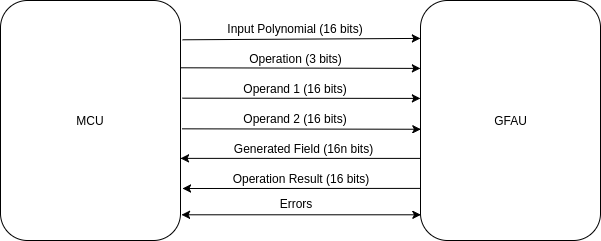
\includegraphics[width=1\textwidth]{system_boundary.png}
                \caption{System Boundary Diagram of the \team~, where $n$ is the Number of Terms} \label{fig:system_boundary}
            \end{center}
        \end{figure}

        \subsection{Data Flow Diagram}
        \begin{figure}[ht]
            \begin{center}
                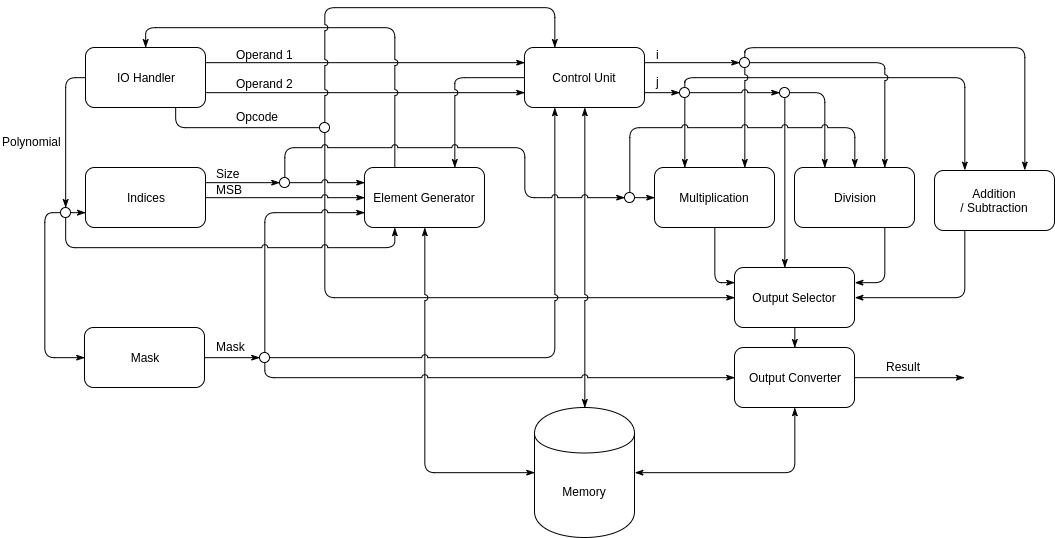
\includegraphics[width=1\textwidth]{data_flow.png}
                \caption{Data Flow Diagram of the \team~} \label{fig:data_flow}
            \end{center}
        \end{figure}


        \subsection{Functional Flow Diagram}


    \section{Requirements}

        \subsection{System Requirements}

        \subsection{Hardware Requirements}


\end{document}
